\chapter{Methodology}\label{chapter:Methodology}
The following chapter in detail explains how the first four steps postulated in the book (\cite{Hyndman.2013}) are used in the forecasting task for this Interdisciplinary Project in detail. Step five, the results and evaluation, is discussed in the next chapters.\newline
\section{Problem Definition}\label{section:Problem Definition}
According to the process, some general questions have to be solved before the forecast is started. For this purpose a stakeholder analysis is done and a SIPOC diagram is created (Table \ref{tab:sipoc}).

\begin{table}[h]
\centering
\caption{SIPOC Diagram derived from the five basic steps}
\label{tab:sipoc}
\scalebox{0.75}{%
\begin{tabular}{|l|l|l|l|l|}
\hline
Supplier                                                                                    & Input                                       & Process                                                          & Output                                 & Customer                                            \\ \hline
\begin{tabular}[c]{@{}l@{}}Emanuel Pallua (COO)\\ Sebastian Sondheimer (BI)\\ Stefan Rothlehner(CTO)\\ Sergej Krauze (CTO)\\ Operations Team\end{tabular} & \begin{tabular}[c]{@{}l@{}}Knowledge\\ Experience\\ Historic Database\end{tabular} & \begin{tabular}[c]{@{}l@{}}Preliminary Analysis\\ Choosing Models\\ Fitting Models\\ Forecasting\\ Evaluating\end{tabular} & \begin{tabular}[c]{@{}l@{}}Forecast\\ Evaluation\\ Result\end{tabular} & \begin{tabular}[c]{@{}l@{}}Emanuel Pallua\\ Sebastian Sondheimer\\ Operation Team\end{tabular} \\ \hline
\end{tabular}}
\end{table}
Emanuel Pallua is identified as the first stakeholder. He is Chief of Operations at VOLO and the one who requested the forecast. His requirement for the forecast is to decrease "waste". Waste is defined as idle times for drivers, like being at the restaurant too early or food losing freshness by lying at the restaurant for too long. Another goal is to save money by maximizing the utilization of drivers and thus decreasing the fleet size. In general he wants a robust forecasting process which can be continuously improved and automated in the future for day to day usage. \newline
The second source and customer in one person is Sebastian Sondheimer who is with Business Intelligence. His aim is to optimize the whole process of VOLO. He supports the forecast process by adding his knowledge of the current key numbers of VOLO. He suggests using only a few performance factors for the forecast. This should include the preparation times of this current slot and day, of the slot in the last seven days and all orders of the last week as well as of the slot and all orders on this weekday of the last four weeks.\newline
As sources on the technical side, there are Stefan Rothlehner and Sergej Krauze, both Chief Technical Officers. Stefan Rothlehner is responsible for the backend database and delivers the data. The information of the orders is extracted from the PostgreSQl database which is hosted on the heroku server. Sergej Krauze who is responsible for the Traveling Salesman Algorithm has the requirement to have the forecast written in Java. Since his work is already in Java and the forecast, once decided that it should be integrated, can be integrated without much additional effort.\newline
The last source and customer is the Operations Team since they are involved in the everyday business. They support the algorithm with their real life scenario knowledge. Their experience is that a 15 minute estimation works reasonably well. In their opinion, a decrease of one third, 33\%, of waste will make it worth to implement the algorithm. In order to have a benchmark for the results of the forecast, the error of their current assumptions will be calculated.
\newline\newline\textbf{Problem Statement}\newline
The goal is to research a forecast for preparation times of meals. The approach should be simple and easy to implement with the Traveling Salesman Algorithm. Reduction of waste should be significant over the current approach.
\section{Gathering Information}\label{section:Gathering Information}
The data for the forecast is taken from the PostgreSQL database of the backend. Every order from the beginning of VOLO in September 2014 has been processed and stored in this database. Each order has a timestamps for each step of the delivery process. This way a rich set of historical data has piled up and is available. For the forecast two data samples are downloaded at different points in time, the training data set and the test data set. The training data set is used to “train” the model and find potential relationships. It creates the first forecast. The result of the forecast is then compared to the result of the test data set. This gives information about the prediction abilities of the model. When the two results are significantly different, the predictive relationships do not hold. The two data sets were dumped on the 26th of March and the 29th of April and contains 3034 and 4973 orders, respectively. The downloaded data sets were saved in comma separated values files, short csv files. Since VOLO was bought and moved to Berlin in April, the company has grown very fast and with it came different problems in operations, e.g. too few expertise or drivers in new cities. In order to have a forecast for a “working” system, only data from the Munich times, when the process was completely supervised by people who had done this for a longer time, was used. New data can be used again when the operations have risen to normality, as observed before the move.\newline
This raw data has some weaknesses. The biggest one is the size of the gathered data, i.e. the lack of data items for some of the categories defined later. Forecasts need big amounts of information to generate a meaningful result. Since some restaurants have too few orders or a lot of bad data for the preparation times, additional expertise has to be put into the forecast. This expertise was taken from the Operation Team. They have to deal with orders on a daily basis and right now have to "forecast" the point in time the driver has to be at the restaurant on their own. In their experience, an estimation of around 15 minutes is a more or less accurate guess for most restaurants except for some which are known for their unpredictability.\newline
In order to use the datasets from the csv files, it has to be parsed into objects in the Java program. For this purpose a csv parser library is used. The library reads the csv file and matches the orders from the database to the OrderModel.class of the code. Not all attributes of the database are used, only the ones related to the forecast are picked from the information. Since there is no tracking in the restaurant for the preparation time, it was decided to take the time interval from the point in time at which the restaurant gets the order transmitted until the driver leaves the restaurant. In the process of volo, the printer in the restaurant prints the recipe at the same time as the driver accepts the delivery, which is saved in the database as \texttt{accepted\_at}. The timestamp of the driver leaving the restaurant is saved in \texttt{delivery\_started\_at}. Since it is not the task to figure out the exact the preparation time but the time from when the order is send to the restaurant and when the driver can pick it up,  these two time stamps can be used, so the clock for the preparation time starts ticking on accepted_at and stops at delivery_started.
\section{Preliminary Analysis}\label{section:Preliminary Analysis}
There are many factors which can influence the preparation times of the restaurant. Some are of external nature, some internal nature. The weather or season can have an effect or if a cook is ill.\newline
Marketing campaigns may boost orders on short time, which can influence the results, but this has not happened in the recorded time frame.\newline
In order to discover these patterns and get a feeling for the data the preliminary analysis is done.
\subsection{Raw Data Cleanup}\label{subsection:Raw Data Cleanup}
First of all the data has be cleaned and a rough overview for the dimensions of the data will be generated. This is done to get a feeling of the time frame a restaurant usually needs to prepare an order. It provides an estimation of what to expect and clue whether the result of a forecast is totally unrealistic or pretty close. In addition to the average time analysis a visualization of the data is done as well. This is done in a time series plot on which it is very easy to see anomalies or patterns of the raw data.\newline

\begin{figure}[h]
\begin{center}
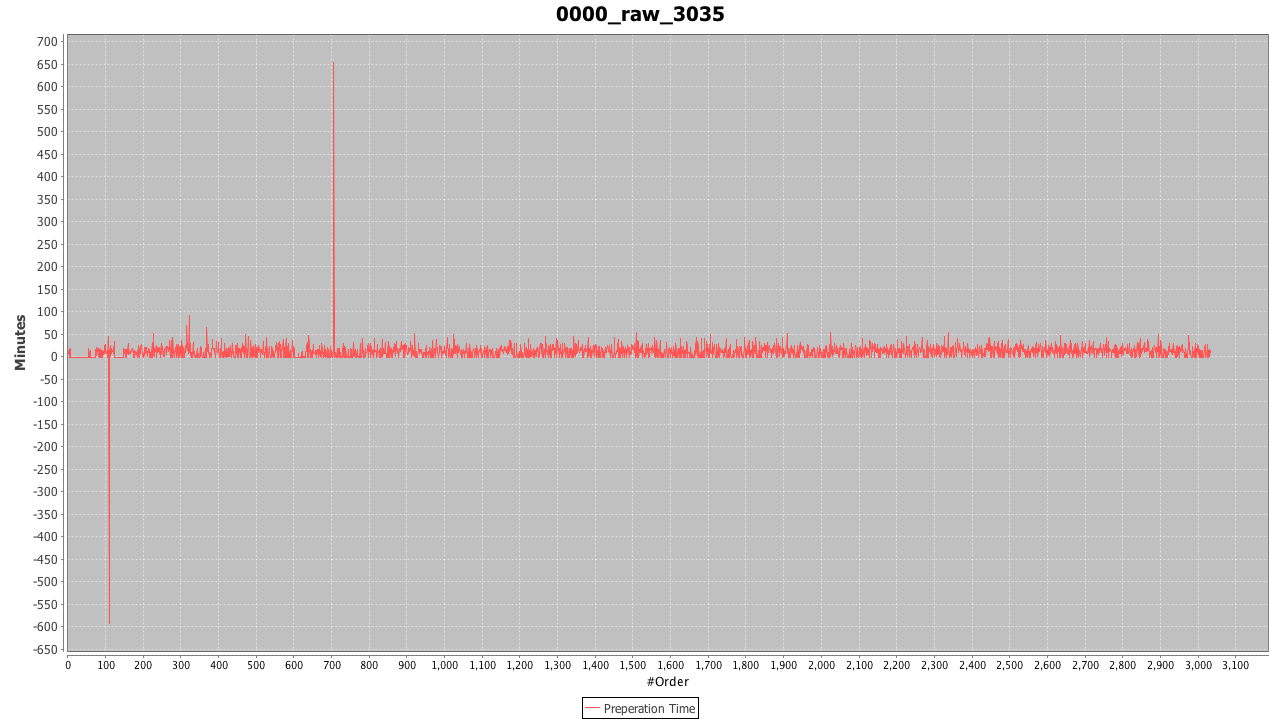
\includegraphics[width=10cm]{images/0000_raw_3035.png}
\caption{Observations of preparation time of all orders without any data clean up}
\label{fig:0000_raw_3035}
\end{center}
\end{figure}

As the first step of the raw data cleanup, the training data is put into a time series graph (Fig. \ref{fig:0000_raw_3035}). This analysis reveals problems in the data. The training data set still contains unfinished orders, bugged orders, which were ended at a wrong point of time, and orders which have corrupted or missing timestamps. Orders of these kinds cannot be transformed correctly and receive a total time of "-1" since either their \texttt{accepted\_at} timestamp is not usable. In case that the orders \texttt{delivery\_started\_at} timestamp is before the \texttt{accepted\_at} timestamp a negative value is visible. This events can be easily spotted in the time series graph and unrealistically reduce the average preparation time to 12 minutes. In order to get realistic results, these flaws in the data set have to be removed. This is done by ignoring all values which are below 0 minutes in the forecast. This action increases the average preparation time to 16 minutes which is much higher than the first result but free of misleading values. The data set which, in contrast to Figure \ref{fig:0000_raw_3035}, does not contain any negative values, is visualised in Figure \ref{fig:0000_invalid_2204}.

\begin{figure}[h]
\begin{center}
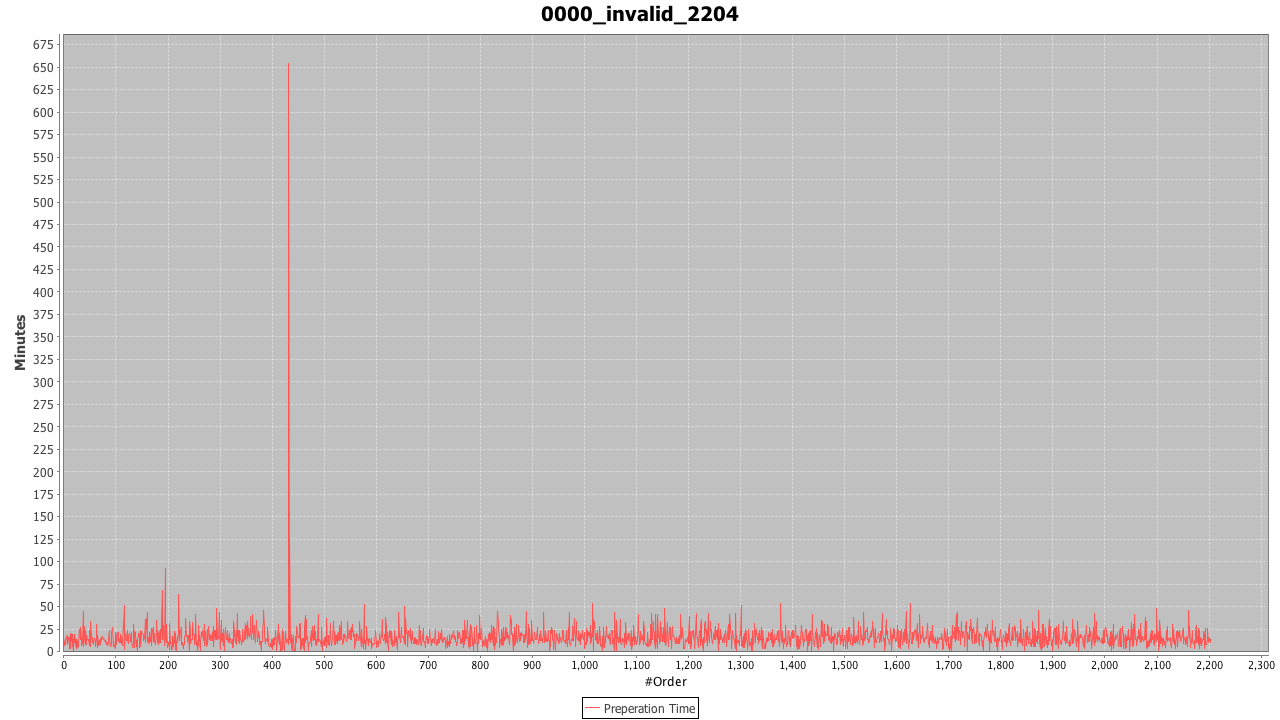
\includegraphics[width=10cm]{images/0000_invalid_2204.png}
\caption{Observations of preparation time of all orders without invalid values}
\label{fig:0000_invalid_2204}
\end{center}
\end{figure}

After removing the obviously unusable orders the data looks a lot more usable. The next problem are the orders which were finished long after they have been started. It has to be assumed that these times were either caused by bugged software or human error in the process. These data points are removed from the data set. For this purpose the Grubbs training for outliers is applied to the dataset and all values that seem not to come from a normally distributed population are removed (\cite{Grubbs}). Figure \ref{fig:0000_grubbed_2201} shows how this action influences the graph. The change can be noted in the scale of the diagram, which is now much more granular. This results in an average preparation time of 15 minutes which is the same result as the operations team suggest to use as a basis.

\begin{figure}[h]
\begin{center}
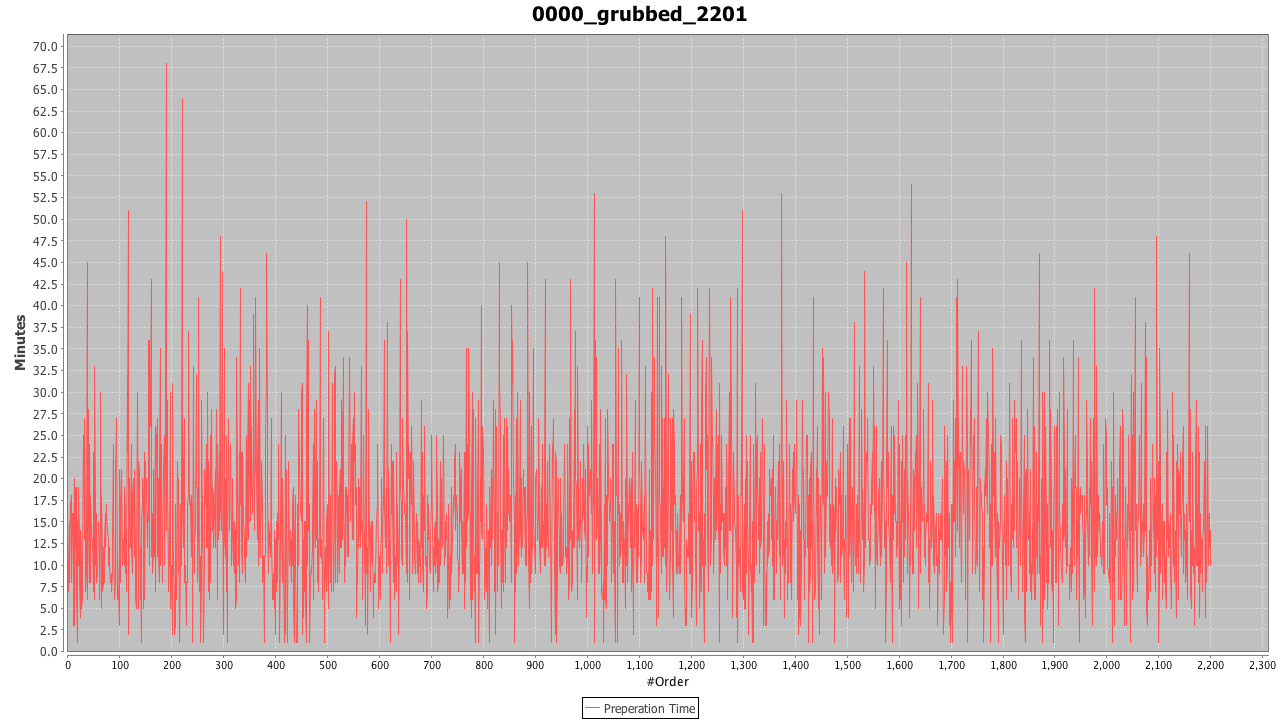
\includegraphics[width=10cm]{images/0000_grubbed_2201.png}
\caption{Observations of preparation time of all orders without invalid values and outliers}
\label{fig:0000_grubbed_2201}
\end{center}
\end{figure}


\subsection{Identifying Patterns}
Now, as only the usable dataset is extracted from the input data, it can be analyzed for patterns, trends or similarities. For this purpose a time component has to be introduced into the graph since putting order after order does not include it.
\subsubsection{Daily Patterns}
As a first try, orders are summed up by day and visualized by average preparation time per day in Figure \ref{fig:0000_byDay_97}. The only usable information that can be extracted is that the average preparation time varies from day to day by up to 19 minutes.

\begin{figure}[h]
\begin{center}
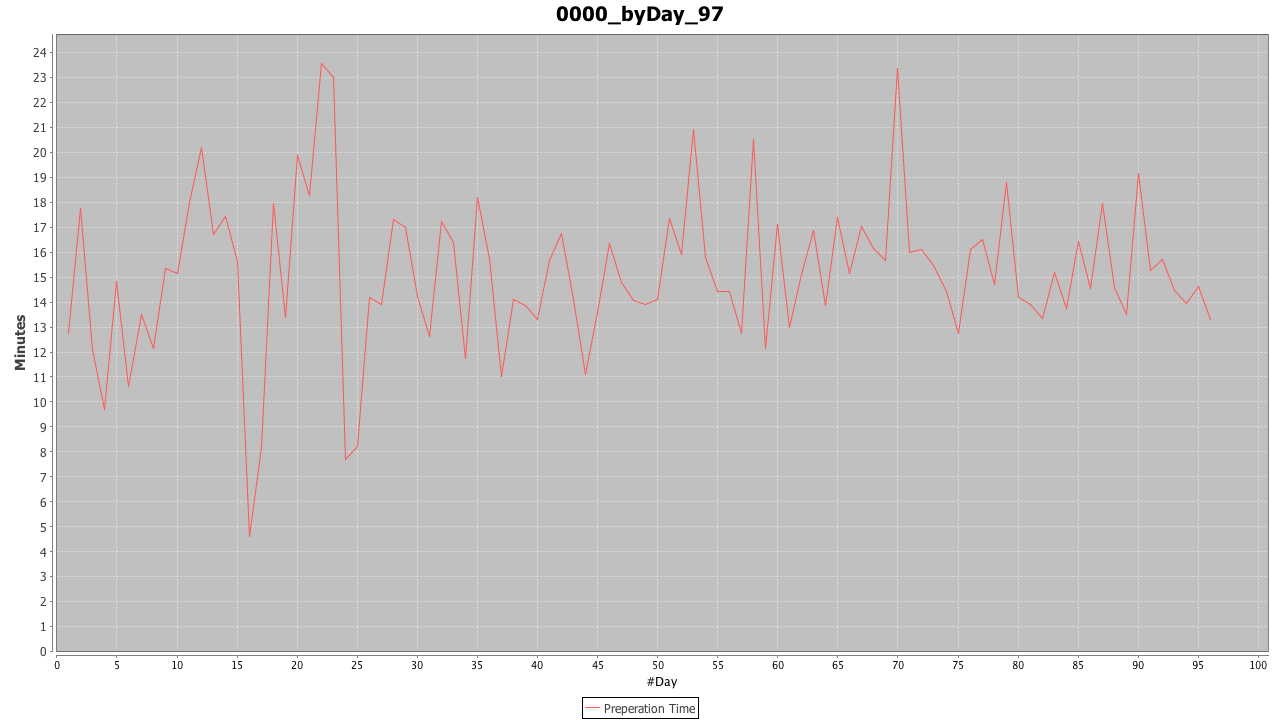
\includegraphics[width=10cm]{images/0000_byDay_97.png}
\caption{Average preparation time per day}
\label{fig:0000_byDay_97}
\end{center}
\end{figure}


No clear trend or pattern can be observed in a day by day time axis diagram (Figure \ref{fig:0000_byDay_97}). In order to inspect behaviour of groups of events in a given category as opposed to single events on the time axis, a box and whisker diagram is created from the data (Figure \ref{fig:triple_boxWhisker}). It shows the median and average preparation time as line and point inside the box. The box represents the upper and lower quartile of preparation times in which 50 \% of the data is while the red whiskers visualize the area without outliers, which are red circles and a red triangle in case they are out of scale. The purpose of this graph is to give an overview of the set of values of the preparation time and the boundaries most of the orders are located in. The data was divided into different categories.\newline
\subsubsection{Week Patterns}
The first diagram in Figure \ref{fig:triple_boxWhisker} on the left is on week basis. It was created to see if there is a trend over time as the company expertise grows. The only observation is that can be made is that after fluctuating preparation times in the first weeks it gets more constant towards the end but there is no clear trend.
\subsubsection{Slot Patterns}
Since no conclusion can be drawn from week analysis, a box whisker diagram for each slot was created (Figure \ref{fig:triple_boxWhisker}, middle). The day is divided into three slots, the big meals, lunch and dinner, as well as the time between these, the afternoon, which is not as busy as the meal times. The diagram shows no real difference in preparation times between the slots. A more in depth analysis has to be done, combining slots with different categories (see below).
\subsubsection{Slot and Weekday Patterns}
Since weekdays can have strong differences in terms of load for the restaurant, a combination of week day and slot needs to be analysed separately (Figure \ref{fig:triple_boxWhisker}, right).
This is done since it contains two different key information. Slots and weekdays alone do not have as much information as the two combined. For example on a sunday evening, many people like to go to a restaurant and do not order, while during the week offices sometimes order big deliveries for lunch. The values in the diagram do not vary much, which can be due to the fact the training set has few values some days.\newline
The difference between slots on weekdays as well as between weekdays is more significant than all other diagrams before and will be considered when creating the model.

\begin{figure}[htp]

\centering
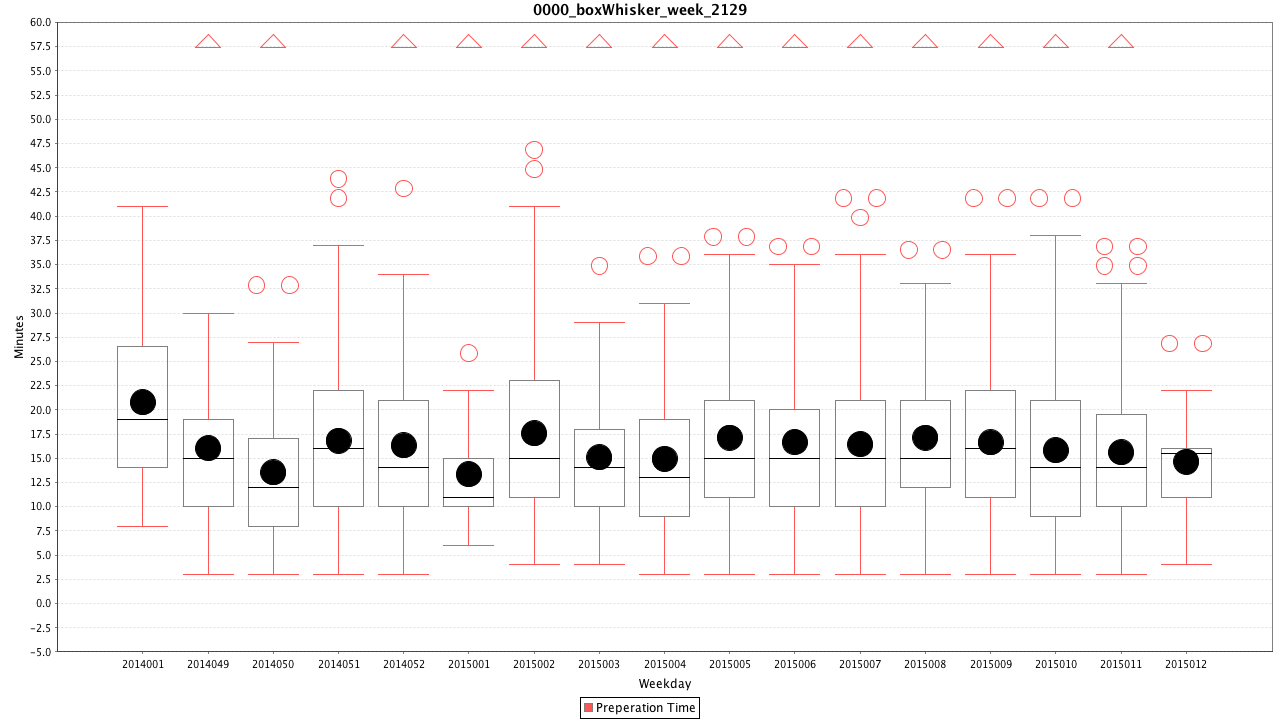
\includegraphics[width=.3\textwidth]{images/0000_boxWhisker_week_2129.png}\hfill
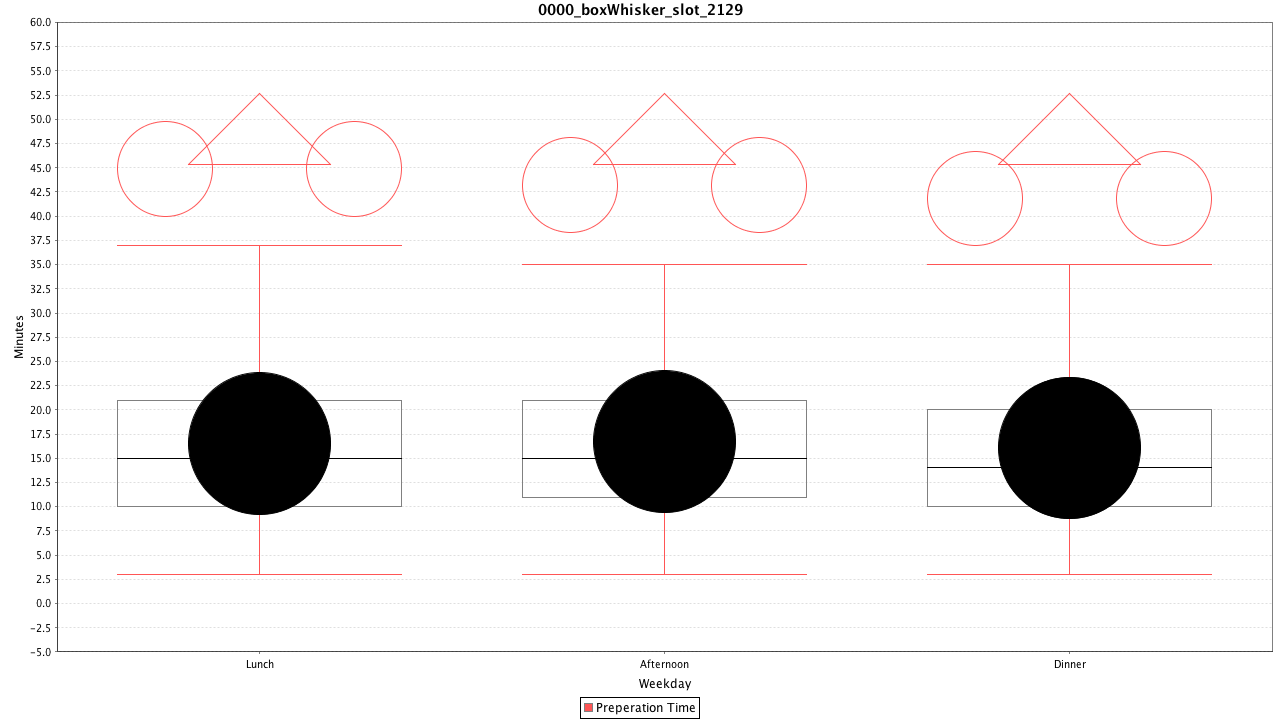
\includegraphics[width=.3\textwidth]{images/0000_boxWhisker_slot_2129.png}\hfill
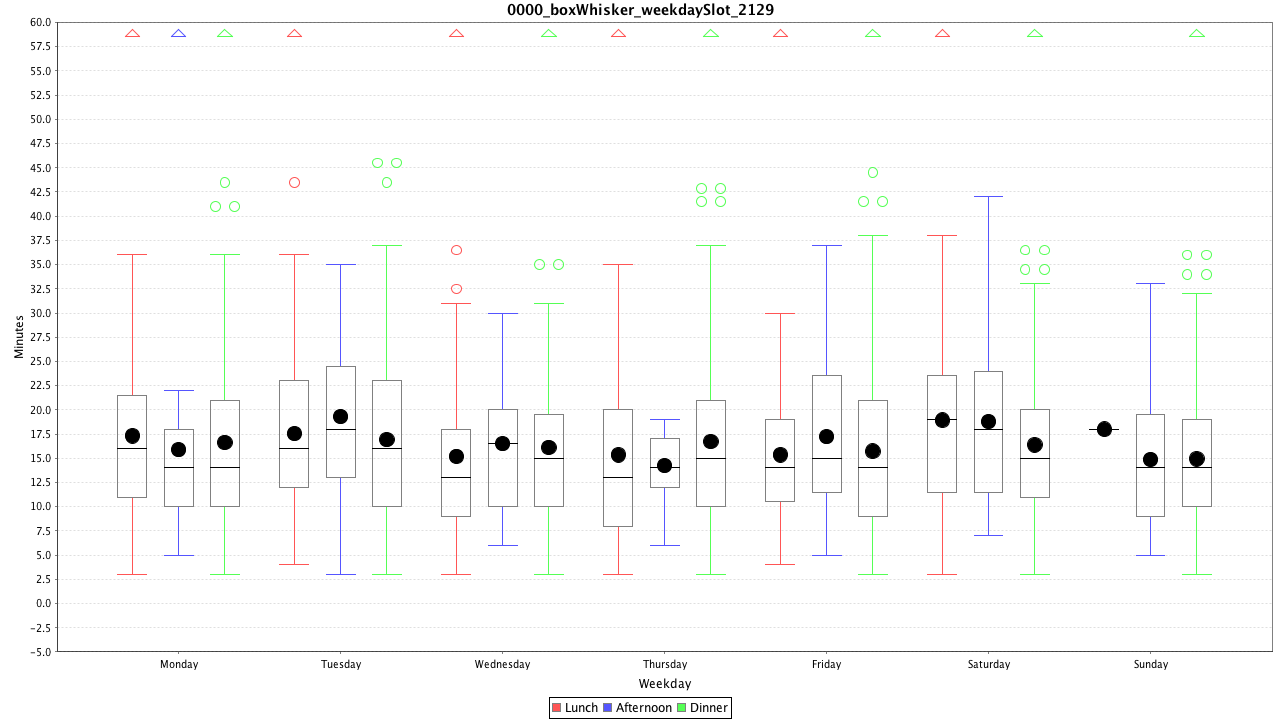
\includegraphics[width=.3\textwidth]{images/0000_boxWhisker_weekdaySlot_2129.png}

\caption{Box Whisker diagrams with different time categorization. By Week (left), by Slot (middle) and by Weekday-Slot (right).}
\label{fig:triple_boxWhisker}

\end{figure}

All these lessons learned from the clean up of the data is also applied to the test data set which is used later.

\subsubsection{Restaurant Patterns}\label{subsection:Restaurant Wise Proceeding}
The restaurants preparation times can be very different. There are restaurants, which have pre-cooked ingredients and others who prepare every meal fresh. Some have simple ways of preparing meals, like sandwiches, while others take long baking, frying or cooking. For all of them, preparation times are different. A roasted duck takes longer than a spring roll.\newline
This suggest looking at each restaurant separately, which initially leads to two categories: One restaurant agnostic and another one restaurant specific. For the evaluation of the restaurant specific forecast yum2take is chosen, as it is the most mature Volo customer with the most data points.\newline
In order to get a first look at the restaurant specific data, a diagram with slot and weekday differentiation is created in Figure \ref{fig:1_boxWhisker_weekdaySlot_686}.
\begin{figure}[h]
\begin{center}
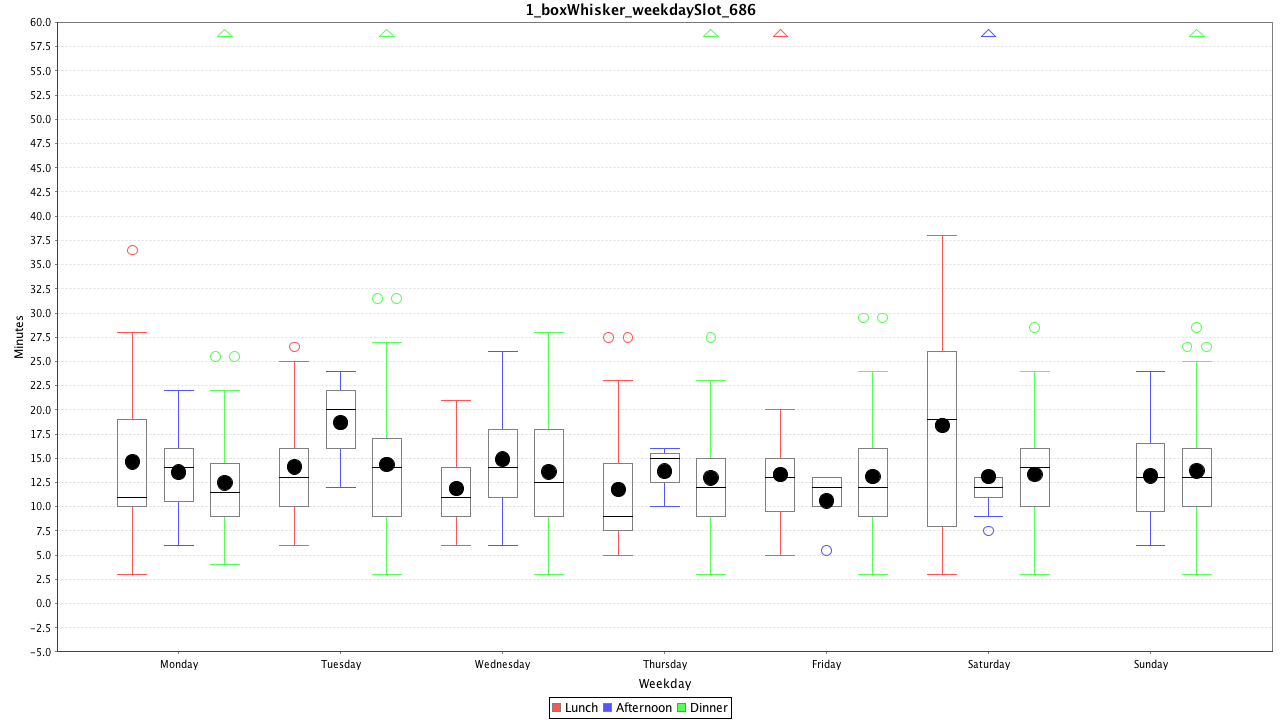
\includegraphics[width=10cm]{images/1_boxWhisker_weekdaySlot_686.png}
\caption{Observations of preparation time of all orders at yum2take without invalid values and outliers}
\label{fig:1_boxWhisker_weekdaySlot_686}
\end{center}
\end{figure}
The distribution in the diagram for yum2take is clearly different from the overall visualization. This confirms the assumption that restaurants should be looked at separately. The average times are also different. Instead of an average of 15 minutes for the preparation of food, the restaurant specific average time for yum2take is 13.1 minutes. This finding should be investigated when creating the models.
\subsection{Current Assumption}
As a stake in the ground and to compare future forecast models do the current process, the RMSE of the current forecasting mechanism where every preparation time is supposed to be 15 minutes is calculated. Based on the training data, it is 8.5 minutes.
\section{Choosing and Fitting Models}\label{Choosing and Fitting Models}
After the preliminary analysis, it is time to fit the data to models for the forecast. A model combines three dimensions, the algorithm, the restaurant category and a time category.
\subsection{Time Categorizing of Orders}\label{subsection:Categorizing by Order}
When categorized by time, only orders in a specific time window are used to calculate the forecast value for the current order. The time window is always relative to the current order. The following time categories were chosen:
\newline\newline\textbf{No Time Categorization}\newline
No time categorization means that for the forecast of the current order all predecessing orders are taken into account. This is done in order to treat all orders the same and get a simple forecast.
\newline\newline\textbf{Day Categorization}\newline
When using day categorization, only the orders before the current one on the same day are used to calculate the forecast value. The day categorization is done since from day to day conditions in the restaurant can change. For instance staff may be ill, delaying meals on that day.
\newline\newline\textbf{Week Categorization}\newline
The week categorization is done to take larger events in account when forecasting, e.g. marketing campaigns. In order to consider such events, this categorization uses all predecessing orders of the calendar week for the calculation.
\newline\newline\textbf{Weekday Categorization}\newline
Weekdays are also different from each other and have to be considered since they cause different utilization of restaurants, e.g. on sundays markets are closed and people tend to order for lunch but go to the restaurant in the evening. For this categorization all orders before the current on this weekday are used for the forecast of the order.
\newline\newline\textbf{Slot Categorization}\newline
In the preliminary analysis three main phases, the slot, were declared as relevant. These slots are lunch, dinner and the time in between and they cause different traffic for the restaurants, lunch and dinner being high traffic while the time in between is not so crowded. In order to consider these day specific differences, it can be applied together with the other time categorizations, to improve the accuracy of the forecast. For example when using day and slot categorization, not all predecessing orders of the current day are considered for the forecast but only the ones in the slot before the current order. The significance of slots has been shown in Figure \ref{triple_boxWhisker}.
\newline\newline\textbf{Single Minislot Categorization}\newline
The minislot categorization divides the day into half hour slots. Since this granularity is finer than the slot categorization, it cannot be combined with it. For each forecast for an order all orders before the current one in this slot are used. This is done to consider short time fluctuations caused by peak times, e.g. the half hour in which most people do their lunch or shortly before eight in the evening before the prime time movie starts.\newline
Even though there might not be enough data for this categorization, is done never the less, to see its potential


\newline\newline\textbf{Edge Case}\newline
Before the actual forecast can be done, the edge case of not having predecessing orders for the current order, has to be resolved. Since the operations teams suggested a 15 minute basic time for preparation, this time is always taken when no forecast value can be generated for the current order.
\subsection{Combination of Time Categorizations}\label{subsection:Categorizing by Order}
Above categorizations can be combined to create a more complex forecasting model. Like all simple models, this complex model is created by using an algorithm and the restaurant category. Only this time a combination of multiple time categories is chosen instead of just one. Each time category is weighted, which is done in 5\% steps, e.g. 5\% category A, 20\% category B and 75\% category C, so all time categories together sum up to 100\%.  This is done for all possible combinations. In order to get a meaningful forecast, the most important time categories are chosen for the model. The time categories are:
\begin{enumerate}
\item Current slot
\item Current day
\item Current slot in the last 7 days
\item Last 7 days in general
\item Slot on the weekday in the last 4 weeks
\item Last 4 weeks in general
\end{enumerate}

The combination of different time categorizations can give information about short term trends, like marketing campaigns, and general long term patterns, like sunday evening is always crowded in the restaurant.\newline
This combination is done to consider the behavior of orders depending on their point in time.
